
In this section, the results obtained from using \texttt{InferPy} to achieve dimensionality reduction of the two given databases to a two-dimensional and a three-dimensional space are reviewed.


\section{Defined models}

The PCA model is defined with the following elements:
\begin{itemize}
  \item The set of i.i.d observed variables \(X_{1},\dots,X_{N}\).
  \item The hidden representation of each variable \(Z_{1}, \dots, Z_{N}\).
  \item A global hidden variable \(\bm{W}\) the linear transformation from one space to the other.
  \item Another global variable \( \delta \) that will allow the model to generate non-centered points.
\end{itemize}

The latent variables prior is a centered Gaussian and the data is supposed to be generated as
\[
     X_n \mid z_n, \bm{w}, \delta \sim \mathcal{N}(\bm{w}^T z_n + \delta, I)
\]
The considered noise value is therefore \(\sigma^{2} = 1\).

\begin{figure}[h!]
  \centering
  \begin{tikzpicture}[
    node distance=1cm and 0.5cm,
    mynode/.style={draw,circle,text width=0.6cm,align=center},
    param/.style={draw,text width=0.5cm,align=center}
    ]

    \node[mynode] (theta) {\(\bm{W}\)};
    \node[mynode, below left=of theta] (zn) {\(Z_{n}\)};
    \node[mynode, ,fill={rgb:black,1;white,2},below right=of theta] (xn) {\(X_{n}\)};
    \node[mynode, above right=of xn] (theta0) {\(\delta\)};


    \plate{} {(zn)(xn)} {\(n = 1\dots N\)}; %
    \path (theta) edge[-latex] (xn)
    (theta0) edge[-latex] (xn)
    (zn) edge[-latex] (xn)
    ;

  \end{tikzpicture}
  \caption{Non-centered Probabilistic PCA model. No noise considered.}
\end{figure}

This model is defined in \texttt{inferPy} as:
\begin{minted}{python}
  @inf.probmodel
  def pca(hidden_dim, observed_dim):
      w = inf.Normal(loc=tf.zeros([hidden_dim, observed_dim]), scale=1, name="w")
      delta = inf.Normal(loc=tf.zeros([observed_dim]), scale=1, name="delta")
      with inf.datamodel():
          z = inf.Normal(tf.zeros([hidden_dim]), 1, name="z")
          x = inf.Normal(z @ w + w0, 1, name="x")
        \end{minted}

The non-linear PCA model is defined using a two-layer neural network, to achieve this, four variables are defined \(\alpha_{0}, \alpha_{1}, \beta_{0}\) and \(\beta_{1}\). All of them following a Gaussian distribution \(\mathcal{N}(0, I)\). The networks output is then computed as

\begin{minted}{python}
  h = tf.nn.relu(z @ beta0 + alpha0)
  return h @ beta1 + alpha1
\end{minted}

This is done to show how \texttt{InferPy} allow networks can be modeled using variables. In the other hand, the variational auto-encoder model is defined using \texttt{Keras} integration with \texttt{InferPy}, so that both networks are defined as an \texttt{inf.layers.Sequential} object.

\section{Results}

\subsection{Mnist}

Firstly, due to the size of the original database, only \(1000\) samples of digits \(1,4\) and \(7\) are used. These are loaded form \texttt{InferPy} directly:

\begin{minted}{python}
  mnist.load_data(num_instances=1000, digits=[1,4,7])
\end{minted}

Function \texttt{print\_class\_pie\_diagram} draws a class pie diagram of the given label set, in this case, their proportions are almost equal (Figure~\ref{fig:mnist_proportion}).

\begin{figure}
  \centering
  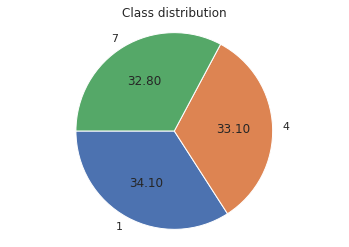
\includegraphics[width = 0.5\textwidth]{tex/images/mnist_proportion.png}
  \caption{Mnist class proportion between numbers \(1, 4\) and \(7\).}\label{fig:mnist_proportion}
\end{figure}

After the inference is done, a sample can be generated from the posterior of a latent variable \(Z\) using the input data:
\begin{minted}{python}
  sample = model.posterior("z", data={"x": X}).sample()
\end{minted}

The function \texttt{print\_posterior} might be used to draw 2D projections of a posterior sample. Results from the 2D reduction are shown in Figure~\ref{fig:mnist_posterior_2D}. In each of the graphics in that figure, projections to each of the learned latent variables are shown, leaving the diagonals to show the density of data-points in the corresponding variable.


\begin{figure}[ht]
  \centering
  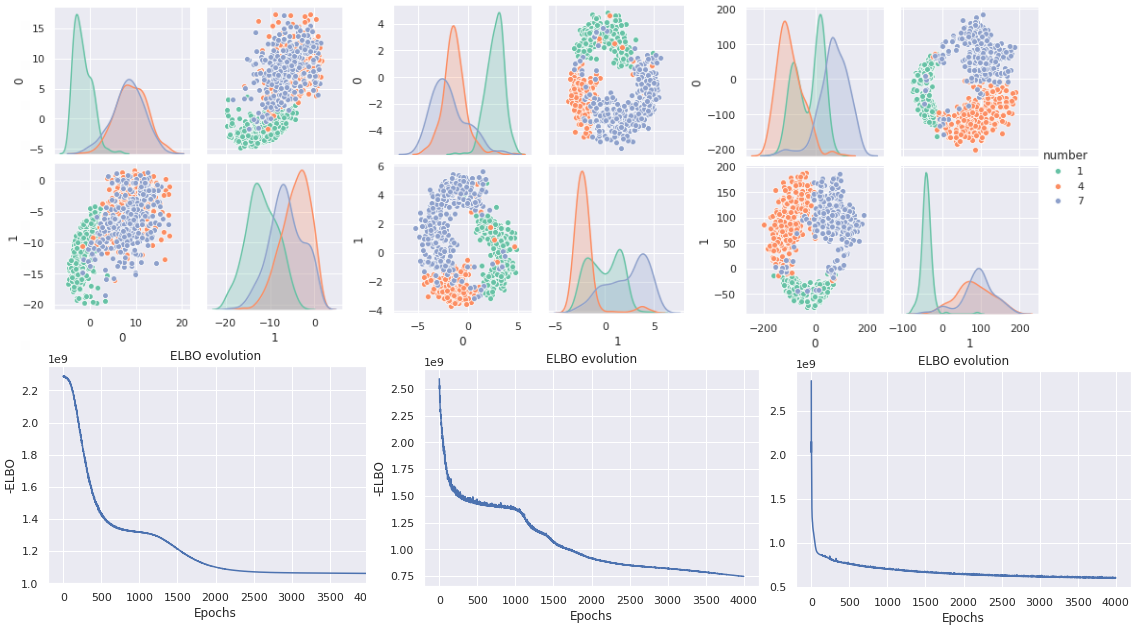
\includegraphics[width = 1\textwidth]{tex/images/mnist_2D.png}
  \caption{PCA, NLPCA and VAE posterior samples and loss functions (from left to right) from Mnist 2D reduction.}\label{fig:mnist_posterior_2D}
\end{figure}

For example in the first image, shown also in Figure~\ref{fig:mnist_pca_2D}, one may see (top left graph) that the first variable (\(0\)) strongly separates samples corresponding to \(1\) from the other samples, whereas the second variable (bottom right graph) (\(1\)) does not make such distinction.

\begin{figure}
  \centering
  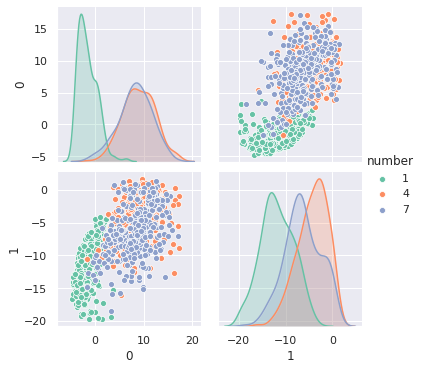
\includegraphics[width = 0.6\textwidth]{tex/images/mnist_pca_2D.png}
  \caption{Projections to each of the two learned variables in Mnist. Diagonals show density over the corresponding diagonal.}\label{fig:mnist_pca_2D}
\end{figure}

The generated representation of the NLPCA and VAE result in a similar ring form, where data samples seem separated between classes. One difference between both results is that the ring scale in the VAE case is bigger (\(200\) compared to \(5\)).

In the 3 cases the loss function (-ELBO) does decrease strongly during the first iteration and slowly during the last ones. This is accentuated in the VAE case (last plot).


In order to test the quality of the reduction, the fact that a good reduction must preserve class separability is used. To test this, the function \texttt{test\_separability} trains a \texttt{Support Vector Machine} from \texttt{Scikit-learn} over both the observed and the reduced space, displaying the score obtained in each one of these. Table~\ref{tab:mnist} shows the obtained results.


\begin{figure}
  \centering
  \begin{tabular}{ccc}
    \hline
    Model    & 2D reduction & 3D reduction \\\hline
    PCA      & 0.737 & 0.916\\
    NLPCA    & 0.947 & 0.969\\
    VAE      & 0.948 & 0.965\\
    \hline
    \hline
    Original data & 0.998 \\
    \hline
  \end{tabular}
  \caption{SVM score.}\label{tab:mnist}
\end{figure}

The three dimensional reduction results are shown in Figure~\ref{fig:mnist_posterior_3D}.

\begin{figure}[ht]
  \centering
  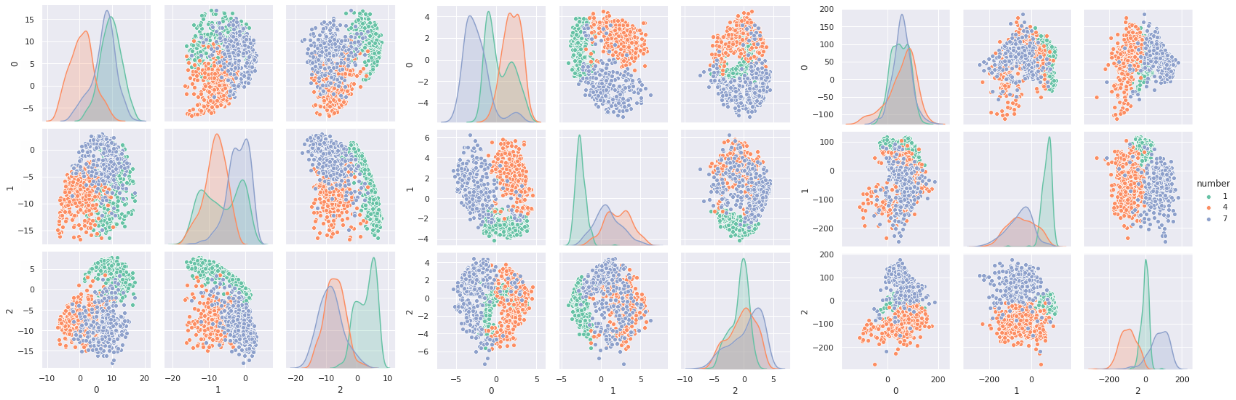
\includegraphics[width = 0.9\textwidth]{tex/images/mnist_3D.png}
  \caption{PCA, NLPCA and VAE posterior samples and loss functions from Mnist 3D reduction.}\label{fig:mnist_posterior_3D}
\end{figure}


\subsection{Breast Cancer Wisconsin}

Firstly, as the given identifier (\(\texttt{id}\)) is a non-predictive variable, it must be dropped from the dataset. Due to the relatively small size to the database, all entries are used in this case.

In this database the class proportion is not balanced at all, Figure~\ref{fig:breast_proportion} shows a dominance of benign entries over the malign ones. Either way, this should not affect the obtained results.

\begin{figure}
  \centering
  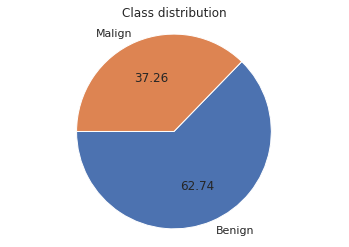
\includegraphics[width = 0.5\textwidth]{tex/images/breast_proportion.png}
  \caption{Breast cancer Wisconsin proportion of malign and benign labels.}\label{fig:breast_proportion}
\end{figure}

In this case, the obtained results from the two-dimensional (Figure~\ref{fig:breast_posterior_2D}) and the three-dimensional (Figure~\ref{fig:breast_posterior_3D}) are quite similar. Where the score table (Table~\ref{tab:breast}) shows very similar results in all cases. However, there are some details worth mentioning that make a difference with the obtained results in \texttt{Mnist}.



\begin{figure}[h]
  \centering
  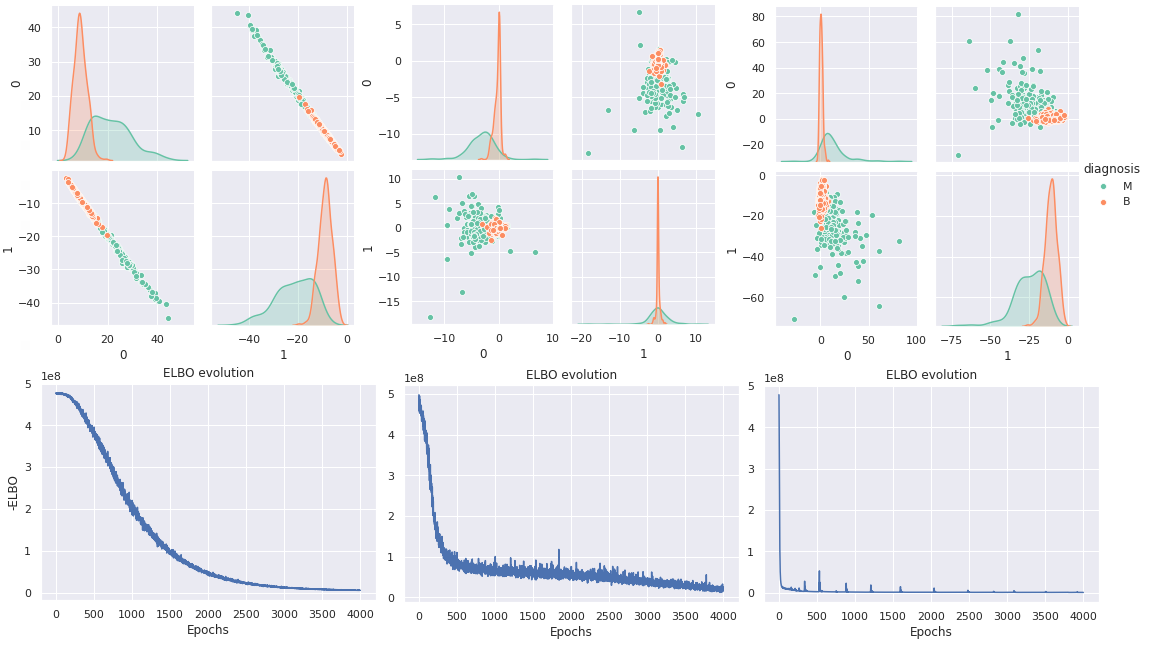
\includegraphics[width = 0.9\textwidth]{tex/images/breast_2D.png}
  \caption{PCA, NLPCA and VAE posterior samples and loss functions from Breast Cancer 2D reduction.}\label{fig:breast_posterior_2D}
\end{figure}

First of all, the results obtained from all models in this database show a highly sharp distribution on the benign entries and a more extended one on the malign one. Secondly, in both reductions, the probabilistic PCA model made a reduction where all the data-points resulted aligned, as a result, these two or three variables are highly correlated, which is not a desired outcome.

In this database, the obtained loss functions present greater oscillations compared to \texttt{Mnist}, which means that the learning task has encountered more local minimum compared to the other database.

\begin{figure}
  \centering
  \begin{tabular}{ccc}
    \hline
    Model    & 2D reduction & 3D reduction \\\hline
    PCA      & 0.9068 & 0.9103\\
    NLPCA    & 0.9121 & 0.9121\\
    VAE      & 0.9349 & 0.9209\\
    \hline
    \hline
    Original data & 0.9226 \\
    \hline
  \end{tabular}
  \caption{SVM score.}\label{tab:breast}
\end{figure}

It is worth mentioning that the separability has being increased (from \(0.9226\) to \(0.9349\)) after reducing to a two-dimensional space using a variational auto-encoder. This ensures that the given reduction does preserve the properties of the database.

There is no big difference between using a two or three dimension in this dataset.

\begin{figure}[ht]
  \centering
  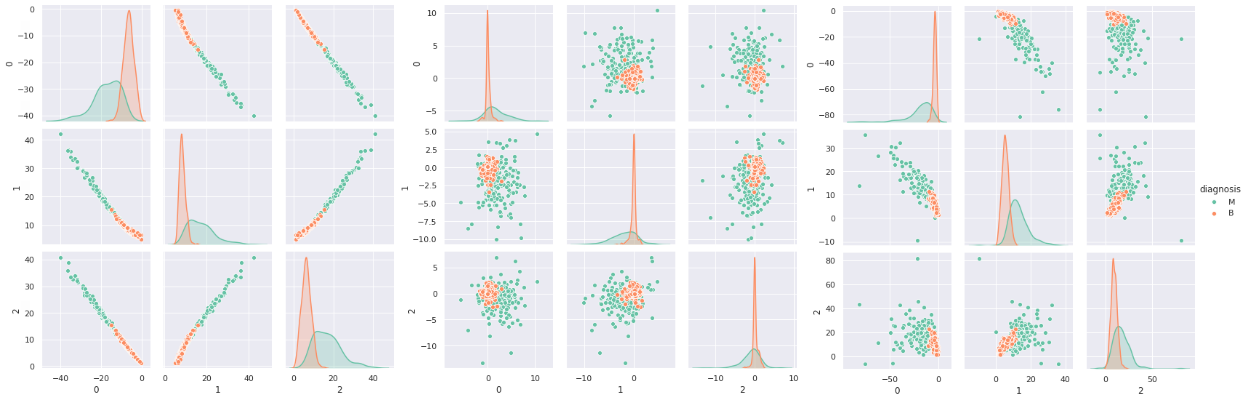
\includegraphics[width = 0.9\textwidth]{tex/images/breast_3D.png}
  \caption{PCA, NLPCA and VAE posterior samples and loss functions from Breast Cancer 3D reduction.}\label{fig:breast_posterior_3D}
\end{figure}

